
\hypertarget{cv:registrarTermino}{\section{Registrar Término de Glosario}} \label{sec:registrarTermino}

	Esta funcionalidad le permitirá registrar un término de glosario dentro del proyecto que se esta operando. 

		\subsection{Procedimiento}

			%Pasos de procedimiento
			\begin{enumerate}
	
			\item Oprima el botón \IURegistrar{} de la pantalla \ref{fig:GestionarGlosario} ''Gestionar Términos de Glosario''.
			
			\item Se mostrará la pantalla \ref{fig:registrarTermino} ''Registrar Término de Glosario''.

			%Pantalla
			\begin{figure}[H]
				\begin{center}
					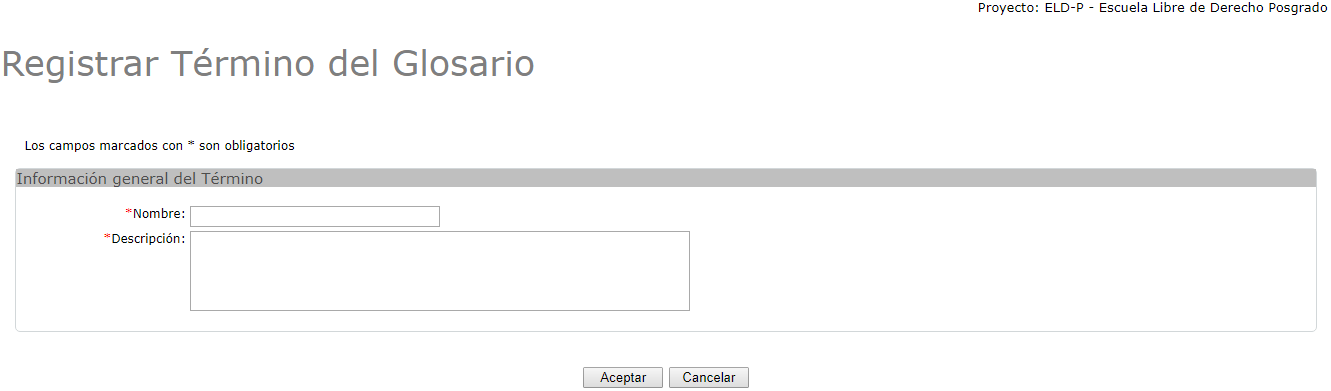
\includegraphics[scale=0.5]{roles/lider/glosario/pantallas/IU6-1registrarTermino}
					\caption{Registrar Término de Glosario}
					\label{fig:registrarTermino}
				\end{center}
			\end{figure}
		
			\item Ingrese el nombre y una pequeña descripción del término de glosario explicando el significado del mismo.
			
			\item Oprima el botón \IUAceptar.
			
			\item Se mostrará el mensaje \ref{fig:terminoRegistrado} en la pantalla \ref{fig:GestionarGlosario} ''Gestionar Términos de Glosario''.
			
			\begin{figure}[htbp!]
				\begin{center}
					
\includegraphics[scale=0.5]{roles/lider/glosario/pantallas/IU6-1MSG1}
					\caption{MSG: Término Registrado}
					\label{fig:terminoRegistrado}
				\end{center}
			\end{figure}
			\end{enumerate}